%------------------------------------------------------------------------------
\chapter{Measurement of top-quark mass}
\label{sec:Temp1}
%------------------------------------------------------------------------------

The event selection and \rm reconstruction are the basis for the final analysis step, which is required to determine the mass of the top-quark. In this final step, the template method  is adopted to determine $m_{\text{top}}$  from Monte Carlo (MC) simulated distributions of observables, which are sensitive to the mass value. These MC simulated samples are generated for different input values of $m_{\text{top}}$ and parametrized with analytical functions, which represent probability densities. These probabilities are used to determine the top-quark mass in an unbinned maximum likelihood fit.

 The template method is a standard analysis tool in high energy physics. However, there are certain issues affecting the measurement of the top-quark mass.  Hence, a unique approach has been developed and applied very successfully for the 7 and 8~TeV measurements~\cite{Aad:2015nba,ATLAS-CONF-2017-071}.

In the following the complete template parametrization is discussed in detail. Furthermore, the likelihood fit and the necessary analysis related assumptions are explained. Finally, the consistency of the fit procedure is tested. 


\section{3D-template method}

The determination of the top-quark mass with the standard template method from simulated distributions as introduced in~\cref{Relevanz}  suffers form large uncertainties, which arise from the imperfect knowledge of the jet energy scale (JES). 
Therefore, a two-dimensional (2D) version of the template method has been developed and successfully  successful applied  by CDF collaboration~\cite{Aaltonen:2011dr}, as well as by the ATLAS collaboration~\cite{ATLAS:2012aj}.



In this measurement,  the top-quark mass is determined together with a global jet energy scale factor (JSF), which is sensitive to JES. 
While in one-dimension, where only $m_{\rm top}$ is measured, the estimator of top-quark mass is stabilised against JES variations, the 2D approach uses in-situ jet scaling~\cite{ATLAS:2012aj}. 
JSF is a multiplicative factor, which is obtained by the deviations of the top-quark mass estimator distribution between simulation and data. The corresponding corrections, which are applied to all jets, are predicted by these observed differences and provide the sensitivity of the JSF to the JES~\cite{ATLAS:2012aj}.

The simultaneous determination of the top-quark mass and the JSF allows to absorb the effects arising from the jet energy scale variations by making use of the multidimensionality of the fit and help to reduce the total systematic uncertainties and especially the systematic uncertainties which arise from the JES. In the 2D ATLAS analysis for example, the JES uncertainty could be reduced form 1.23~GeV to 0.66~GeV and the total systematics from 2.66~GeV to 2.39~GeV~\cite{ATLAS:2012aj}.  

The largest systematic uncertaintes in the 2D template fit arise form the $b$-to-jet energy scale (bJES). Therefore, the 2D template approach has been extended to three-dimensional (3D) template fit for the 7~TeV~\cite{Aad:2015nba} and the 8~TeV~\cite{ATLAS-CONF-2017-071} measurement and is the base for this analysis. Equal to the JSF a $b$-to-jet energy scale factor (bJSF) is introduced, which is sensitive to bJES  and simultaneously determined with the top-quark mass and JSF. 
 The large impact of the JES uncertainties on the top mass measurement has been shown by previous top-quark mass measurements.
 The results of both 3D measurements demonstrate clearly the impact of the jet energy scales.
  For  the 7~TeV analysis, the JES uncertainty is with 0.58 $ \pm $ 0.11~GeV~\cite{Aad:2015nba} one of the largest systematics, as well as for  the 8~TeV measurement, where the JES uncertainty is 0.54 $\pm$ 0.11~GeV~\cite{ATLAS-CONF-2017-071}.

However,  the success of the three dimensional approach can also be  seen for example by the remarkable results from the 8~TeV measurement.  The achieved improvement of a two dimensional fit, i.e. the determination of $m_{\text{top}}$ and JSF, compared to a one dimensional fit where only $m_{\text{top}}$ is measured, is  8.3~\% of the final error on $m_{\text{top}$~\cite{ATLAS-CONF-2017-071}.
Moreover, the additional measurement of  bJSF improves the total uncertainty about 43~\%~\cite{ATLAS-CONF-2017-071}.
 Despite these impressive results, one has to keep in mind that the situation might be different for the 13~TeV analysis and a judging statement can only be given after the first evaluation of all uncertainties.

In order to measure the top-quark mass and both jet scale factors, estimator distributions have to be established which are sensitive to these three quantities. In this analysis, the three estimators are obtained via the event reconstruction and have already been introduced in~\cref{ch5} and are the same as for the previous measurement. 
 
The first estimator is the  reconstructed top-quark mass $m_{\text{top}}^{\rm reco}$, which is obtained from the kinematic likelihood fit of the event reconstruction.
From the corresponding  jet permutation of the \textsc{KLFitter} output, the reconstructed $W$-boson mass $m_{\text{W}}^{\rm reco}$ is used, as well as the third variable $R_{\text{bq}}^{\rm reco}$. While $m_{\text{top}}^{\rm reco} $ is determined as free parameter of the kinematic likelihood fit,  the other two are built from the original four vectors.  $R_{\text{bq}}^{\rm reco}$ is here calculated with the two $b$-tag definition. 

For all three of these reconstructed estimators, Monte Carlo simulated distributions are generated, with an input top-quark mass value between 170.0 and 175.0~GeV. The nominal sample has a mass of 172.5~GeV. Furthermore, all of these distributions are calculated for different scale factors. 
If the JSF is varied (between 0.96 and 1.04) the bJSF is set to unity and vice versa.

For the choice oft the three estimators is based on the sensitivities to the top-quark mass and the jet scale factors, since these are essential for this measurement.  
 In~\cref{fig:Comparison} the sensitivities of the estimator distributions for different values for $m_{\text{top}}$, JSF and bJSF are shown and compared to 
the nominal sample (red). For each sample, only one variable is varied, while the rest is set to the nominal values, which is 172.5~GeV for $ m_{\text{top}}$ and 1.00 for both scale factors. The deviations from the nominal samples are displayed in the ratio plot below. 
As it can be seen in~\cref{fig:mtopmtop,fig:mtopJSF,fig:mtopbJSF}, the first estimator  $m_{\text{top}}^{\rm reco}$  shows a noticeable sensitivity to all three variables, which one expect since the jet energy scales, which are considered by jet energy scale factors, affect the measurement of the top-quark mass noticeable. 
In the second line the sensitivities of  $m_{\text{W}}^{\rm reco}$ are displayed. As it can be seen, the reconstructed $W$-boson mass  only varies with the jet energy scale factor (JSF) (see~\cref{fig:mwmtop,fig:mwJSF,fig:mwbJSF}). This is in good agreement with the expectations, since $m_{\text{W}}^{\rm reco}$ is calculated as the invariant mass, which only takes the light-jets of the hadronically decaying $W$-boson into account. 



The third estimator distribution $R_{\text{bq}}^{\rm reco}$ (~\cref{fig:Rbqmtop,fig:RbqJSF,fig:RbqbJSF}), however, shows a weak sensitivity to JSF variations and a larger one to the variations of the bJSF. 
The sensitivity to the bJSF is realized by the enumerator in the $R_{\text{bq}}^{\rm reco}$ definition, where the transverse momenta of the $b$-jets are included, while the scalar sum in the denominator respects the transverse momenta of the light jets of the $W$-boson.


The scale factors are  multiplicative quantities and reduce or increase the number of events  passing the event selection cuts. Events with a higher scale factor, compared to the nominal one, are more likely to pass the event selection than those from samples with a lower scale factor. This can explains the observed shifts in the displayed distributions.

 Furthermore, the displayed distributions in~\cref{fig:Comparison} are already normalized to one and parametrized with analytical functions, which are basically the sum of  Gaussians and Landau distributions
 
 The parametrization of the templates is one of the major tasks of this thesis. This part has been implemented completely new, based on the method of the previous measurements. 

In the following the different steps of the template parametrization are introduced together with corresponding results. If not mentioned otherwise, all shown distributions are normalized to one. 



\begin{landscape}
	

\begin{figure} % "[t!]" placement specifier just for this example
	\centering 
	

	\begin{subfigure}{0.37\textwidth}
		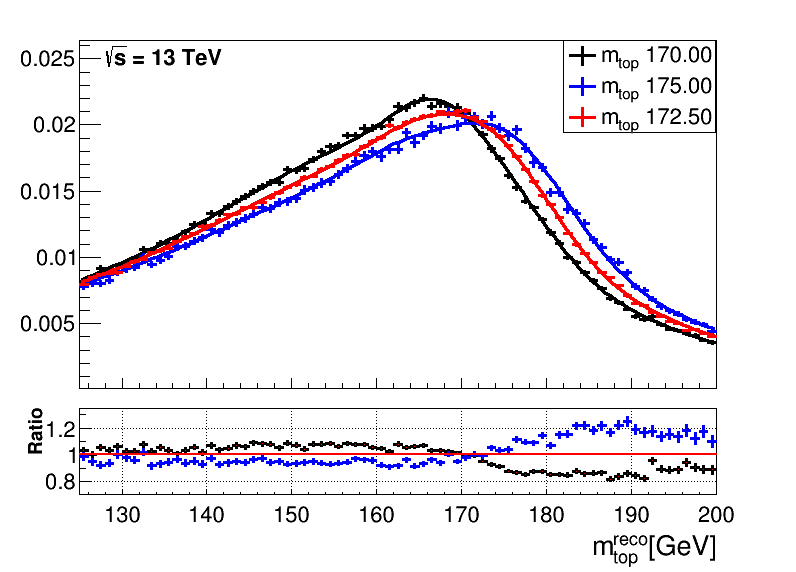
\includegraphics[width=\linewidth]{Pics/PlotCombi/mtop_mtop.png}
		\caption{$m_{top}^{reco}$ vs $m_{top}$} \label{fig:mtopmtop}
	\end{subfigure}
	\hspace*{0.25cm}
	\begin{subfigure}{0.37\textwidth}
	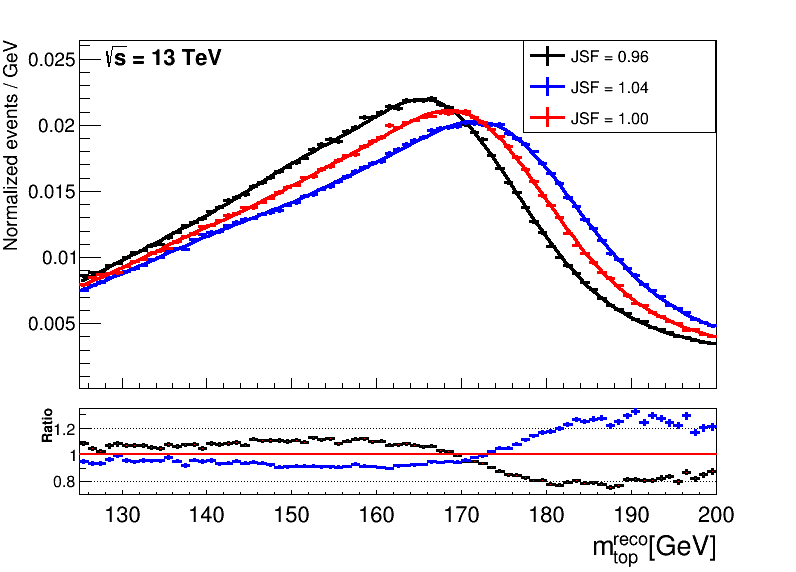
\includegraphics[width=\linewidth]{Pics/PlotCombi/mtop_JSF.png}
	\caption{$m_{top}^{reco}$ vs JSF} \label{fig:mtopJSF}
	\end{subfigure}
	\hspace*{0.25cm}
	\begin{subfigure}{0.37\textwidth}
	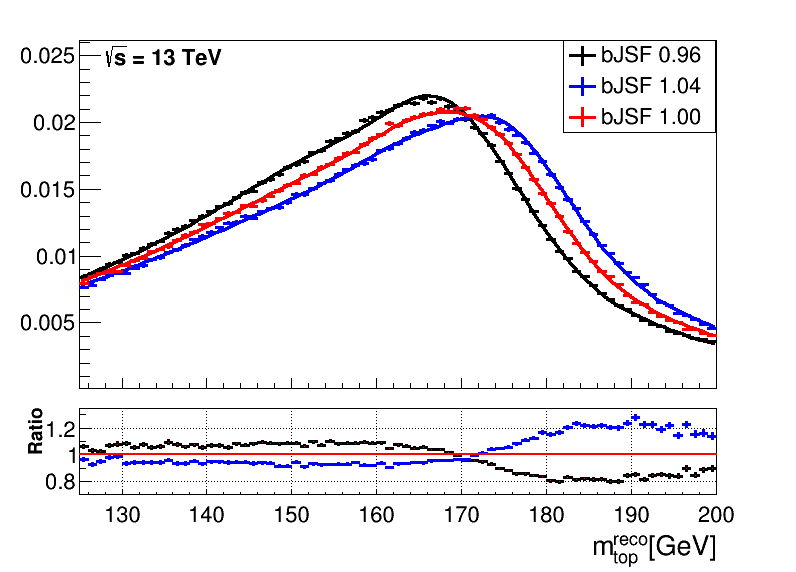
\includegraphics[width=\linewidth]{Pics/PlotCombi/mtop_bJSF.png}
	\caption{$m_{top}^{reco}$ vs bJSF} \label{fig:mtopbJSF}
	\end{subfigure}
	\begin{subfigure}{0.37\textwidth}
	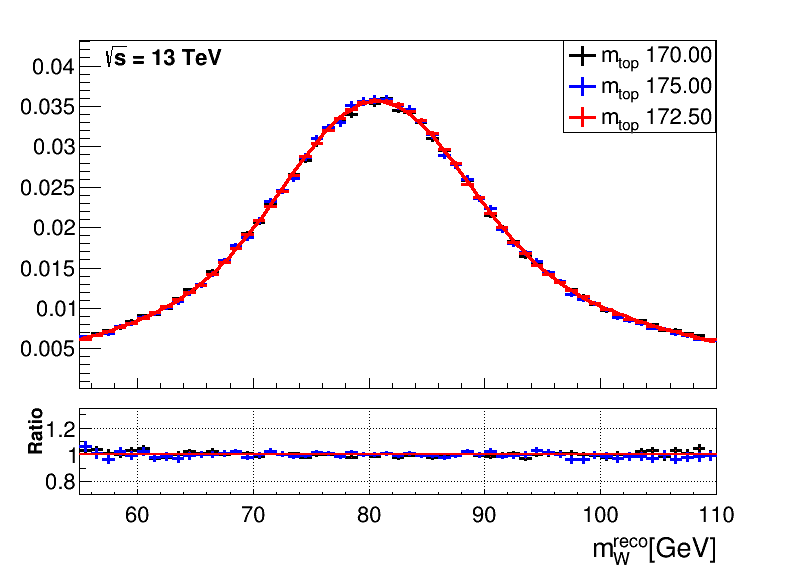
\includegraphics[width=\linewidth]{Pics/PlotCombi/mw_mtop.png}
	\caption{$m_{W}^{reco}$ vs $m_{top}$} \label{fig:mwmtop}
	\end{subfigure}
	\hspace*{0.25cm}
	\begin{subfigure}{0.37\textwidth}
	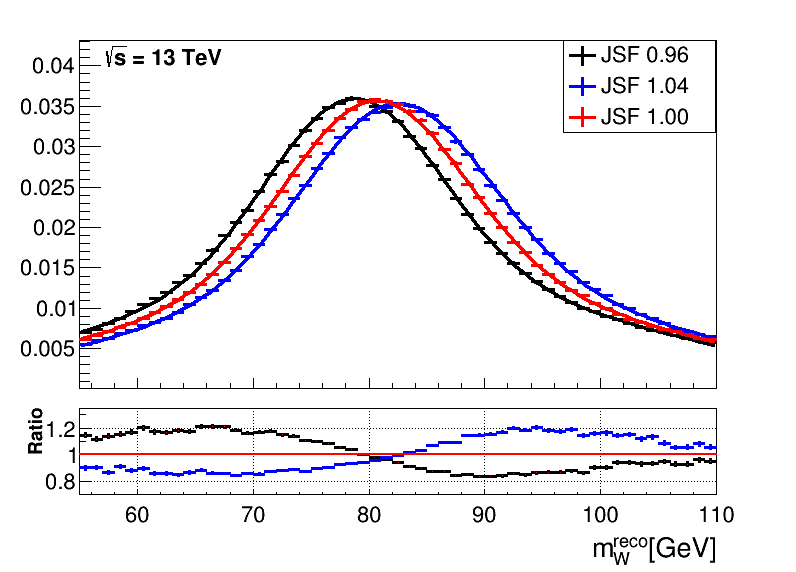
\includegraphics[width=\linewidth]{Pics/PlotCombi/mw_JSF.png}
	\caption{$m_{W}^{reco}$ vs JSF} \label{fig:mwJSF}
	\end{subfigure}
	\hspace*{0.25cm}
	\begin{subfigure}{0.37\textwidth}
	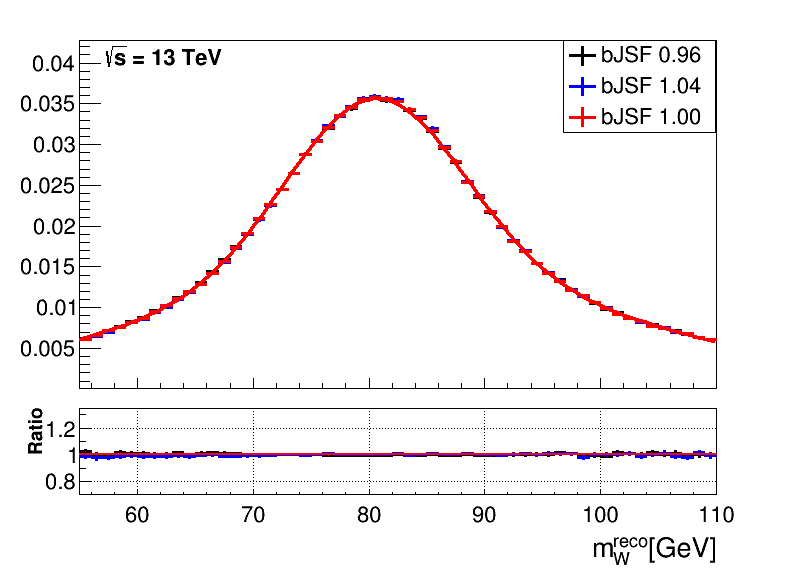
\includegraphics[width=\linewidth]{Pics/PlotCombi/mw_bJSF.png}
	\caption{$m_{W}^{reco}$ vs bJSF} \label{fig:mwbJSF}
	\end{subfigure}
	\begin{subfigure}{0.37\textwidth}
	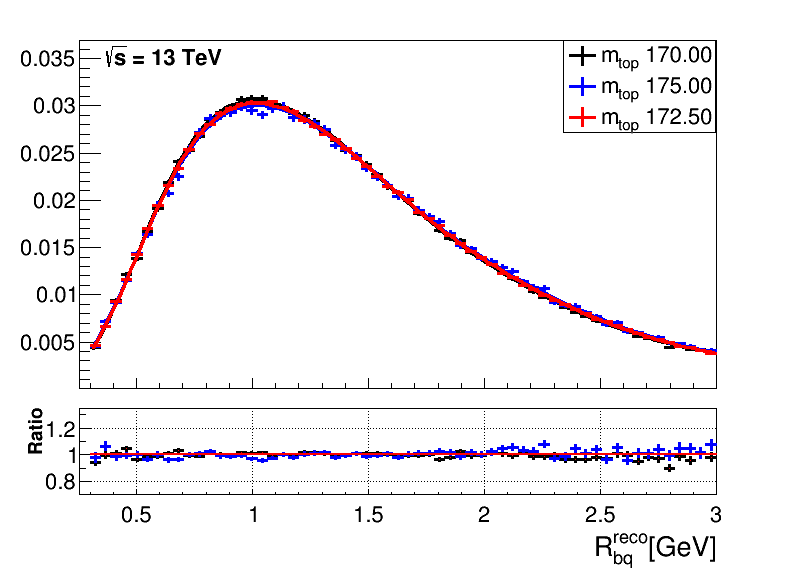
\includegraphics[width=\linewidth]{Pics/PlotCombi/rbq_mtop.png}
	\caption{$R_{bq}^{reco}$ vs $m_{top}$} \label{fig:Rbqmtop}
\end{subfigure}
\hspace*{0.25cm}
\begin{subfigure}{0.37\textwidth}
	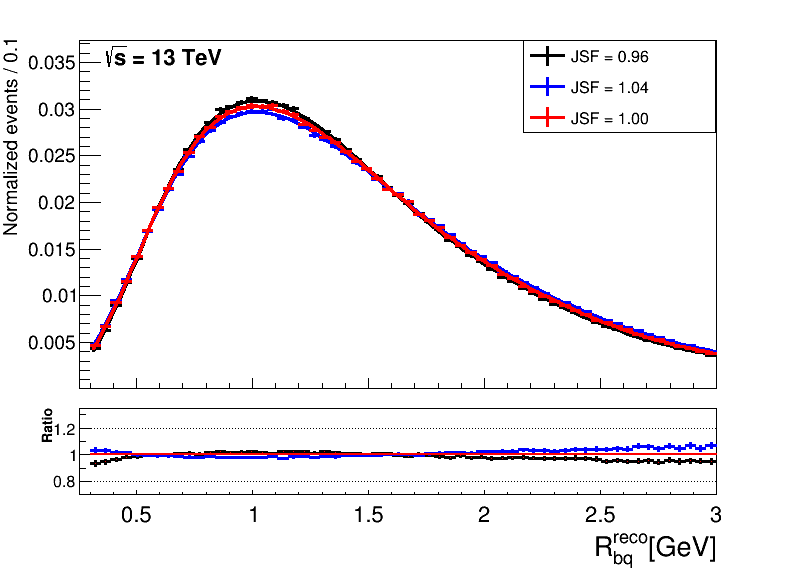
\includegraphics[width=\linewidth]{Pics/PlotCombi/rbq_JSF.png}
	\caption{$R_{bq}^{reco}$ vs JSF} \label{fig:RbqJSF}
\end{subfigure}
\hspace*{0.25cm}
\begin{subfigure}{0.37\textwidth}
	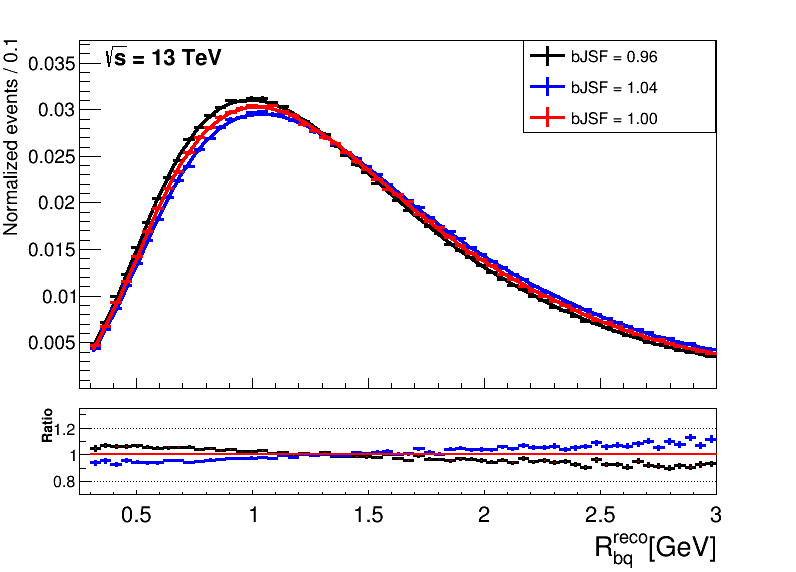
\includegraphics[width=\linewidth]{Pics/PlotCombi/rbq_bJSF.png}
	\caption{$R_{bq}^{reco}$ vs bJSF} \label{fig:RbqbJSF}
\end{subfigure}
	\caption{Comparison of signal $t\bar{t}$ templates for different simulated top-quark masses and scale factors. For each of the three observables, ($m_{top}^{reco}$, $m_{W}^{reco}$ and $R_{bq}^{reco}$) the sensitivities are displayed, by overlaying the nominal (red) sample with samples for different JSF, bJSF and $m_{top}$ . The unvaried quantity is kept to the nominal value. }
\end{figure}\label{fig:Comparison}	
\end{landscape}
  
  

\subsubsection{The template parametrization}


The parametrization of the estimator distributions consists of several sub-steps. Firstly, the actual parametrization, which is used to obtain the probability densities, is performed. The procedure is briefly as follows: 
\begin{itemize}
	\item First of all, each single distribution is fitted with the analytical functions described below to obtain a set of parameters ($p_i$ with $i$ =0,1,...).
	\item The fitted parameters are parametrized as linear functions of $m_{\text{top}}$, JSF and bJSF. 
	\item With parameters from the two steps above, as initial values, a combined fit is performed to obtain the final parametrization of the templates.
\end{itemize}   

 
 In the case of this thesis,  only templates of signal events are used to perform a first test of the method. However, the major changes which have to be considered for the inclusion of the background samples are also taken into account in following.  


\subsubsection{The single fits}  


 At the beginning of the parametrization process, the best possible initial conditions are searched for the  combined fit of the templates. Furthermore, one is also interested in the dependencies between the three estimators ($m_{\text{top}}^{\rm reco}$, $m_{\text{W}}^{\rm reco}$ and $R_{\text{bq}}^{\rm reco}$) and the three observables, which are of interest ($m_{\text{top}}$, JSF and bJSF). Therefore, two interpolation steps are performed. 

 First of all, each single \rm reconstructed template is fitted with an  analytical function. For  $m_{\text{top}}^{\rm reco}$  and  $m_{\text{W}}^{\rm reco}$, this is the sum of a Gaussian, a normal Landau function and a mirrored Landau function.  $R_{\text{bq}}^{\rm reco}$ is fitted with the sum of two gaussians and one Landau distribution. 
Since $m_{W}^{\rm reco}$ does not show any significant sensitivities on $m_{\text{top}}$ and bJSF, only the samples with different JSF are parametrized. 
In the analysis published in~\cite{ATLAS-CONF-2017-071}, the $m_{\text{W}}^{\rm reco}$ distribution was parametrized  by the sum of two Gaussians. In this thesis however it has been found that the sum of a Gaussian, a Landau and a mirrored Landau distribution describes the observable better.

In general different functions for the parametrization can be used, since there is no need for physical motivation of the selected functional forms. The interest is only on a good shape description of the
 estimator distributions. Therefore, 
 
 The so-called crystall-ball function, might for example be a good alternative for the description of $m_{\text{top}}^{\rm reco}$ and $m_{\text{W}}^{\rm reco}$ seems to agree well with the shape of a Breit-Wigner distributions, which was explicitly tested during this master project.  
Despite this interesting possibilities, main goal for this theses has been to be as consistent as possible with the previous measurements, in order to make it easy to compare the results.  

 From the first parametrization steps nine parameters ($p_i$) are obtained for each fitted sample of all three distributions ($m_{\text{top}}^{\rm reco}$, $m_{\text{W}}^{\rm reco}$ and $R_{\text{bq}}^{\rm reco}$). The  parameters  represent the amplitude, the mean and the standard deviation of the fit functions. The detailed assignment of the functions can be found in~\cref{tab:parameters}. All parameters of the different sets with same index $i$  are plotted against the simulated $m_{\rm top}$, JSF and bJSF of the corresponding sample. The plots are parametrized with linear functions.  Each parameter ($p_i$) can then be written in the following form:
\begin{eqnarray}
&&p_i = a_{\rm 0i} + a_{\rm 1i} m_{\text{top}}, \nonumber \\
&& p_i = b_{\rm 0i} + b_{\rm 1i}(\text{JSF} - 1.00) \hspace{0.5cm}     \text{and}      \nonumber \\   
&& p_i = c_{\rm 0i} + c_{\rm 1i}(\text{bJSF - 1.00}). \nonumber    \\
\end{eqnarray}
The parameters are described by the slope and the offset of the linear functions. All parameters which are determined in these two steps  are used  as initial parameters  for the combined template parametrization.

\begin{center}
	\captionof{table}{Assingment of the fit paramertes and the analytical functions. $A$ denotes the amplitude of the function, $\mu$ the mean and $\sigma$ the standard deviation.}\label{tab:parameters}
	
	
	
	\vspace{0.3cm}	
	\begin{tabular}{>{}m{3.0cm}>{}m{3.0cm} >{}m{3.0cm}>{}m{3.0cm} } \toprule
		
		Parameter&   $m_{\text{top}^{reco}}$&  $m_{\text{W}^{reco}}$ & $R_{\text{bq}^{reco}}$\\
		\midrule
		$p_0$ & $A$ Gaussian& $A$ Gaussian &$A$ Gaussian 1\\
		$p_1$ &  $\mu$ Gaussian& $\mu$ Gaussian & $\mu$ Gaussian 1\\
		$p_2$ &  $\sigma$ Gaussian& $\sigma$ Gaussian&$\sigma$ Gaussian1\\
		$p_3$ & $A$ Landau            & $A$ mirrored Landau &$A$ Gaussian 2\\
		$p_4$ &  $\mu$ Landau      & $\mu$ mirrored Landau& $\mu$ Gaussian 2\\
		$p_5$ &  $\sigma$ Landau   & $\sigma$ mirrored Landau&$\sigma$ Gaussian 2 \\
		$p_6$ & $A$ mirrored Landau & $A$  Landau}&$A$ Landau\\
	$p_7$ &  $\mu$ mirrored Landau& $\mu$ Landau& $\mu$ Landau\\
	$p_8$ &  $\sigma$ mirrored Landau& $\sigma$ Landau&$\sigma$ Landau\\
	
	\bottomrule
		\vspace{1.0cm}	
\end{tabular}

\end{center}

\begin{figure} % "[t!]" placement specifier just for this example
	\centering 
	
	
	\begin{subfigure}{0.45\textwidth}
		\includegraphics[width=\linewidth]{Pics/Linear/{Lin0_d0_p2_n}.png}
		\caption{$m_{\text{top}}^{\rm reco}$ P2 vs $m_{\text{top}}$} \label{fig:lin1}
	\end{subfigure}
	\hspace*{0.2cm}
	\begin{subfigure}{0.45\textwidth}
		\includegraphics[width=\linewidth]{Pics/Linear/{Lin0_d1_p1_n}.png}
		\caption{$m_{\text{W}}^{\rm reco}$ P1 vs JSF} \label{fig:lin2}
	\end{subfigure}

	\begin{subfigure}{0.45\textwidth}
	\includegraphics[width=\linewidth]{Pics/Linear/{Lin0_d2_p3_n}.png}
	\caption{$R_{\text{bq}}^{\rm reco}$ P3 vs bJSF} \label{fig:lin3}
\end{subfigure}
	\caption{Linear parametrization $p_i$ of the parameters, obtained by the single template fits. Selected parameters are fitted against the different simulated values of $m_{\text{top}}$ and the scale factors. For the scale factors, only the differences from the nominal value $\Delta$, are displayed.}\label{fig:linear1}
\end{figure}



 In~\cref{fig:linear1} examples of the linear parametrization of the fitted parameters, which belong to the single template fit, are shown. The parameters of the different individual $m_{\text{top}}^{\rm reco}$ template fits are plotted against the simulated top-quark mass, and the different JSF and bJSF.  In analogy, there are linear parametrizations of the same kind for  $R_{\text{bq}}^{\rm reco}$, while for $m_{\text{W}}^{\rm reco}$ there is only a linear fit in terms of the jet energy scale JES. The linear dependencies between the parameters of the estimator fits and the observables are essential for the analysis. This will become more clearly below with the introduction of the simultaneous parametrization. Only if the distributions are well described and the linearity of each parameter has been achieved, the results of the single fits can be used to perform the simultaneous fit to the estimator distribution. 

 The complete linear fit of all  parameters and the corresponding plots can be found in~\cref{sec:apptem}. In order to achieve a satisfying result, some parameters are fixed, this can be seen by the fact that the linear fit results in a constant straight line.







\subsubsection{Simultaneous template parametrization }

With the parameters obtained by the previous parametrization steps, three  final  fits are performed.  For example, all  $m_{\rm top}^{\rm \rm reco}$ distributions  are used in a single combined fit. The same procedure is performed for all  $m_{\rm W}^{ \rm \rm reco}$ and $R_{\rm bq}^{\rm \rm reco}$ distributions.
The key ingredients for the combined parametrization of the templates are the linear dependencies, between the different parameters of the fit functions and the three variables $m_{\text{top}}$, JSF and bJSF, which are used  for a sub-parametrization of the parameter set  $p_i$ of the analytical fit functions:
\begin{equation}\label{eq:lin}
p_i = a_{\rm 0i} + a_{\rm 1i}m_{\text{top}} + a_{\rm 2i}(\text{JSF}-1.00) + a_{\rm 3i}(\text{bJSF}-1.00) .
\end{equation}
For the \rm reconstructed $W$-boson mass, the parametrization  is adopted by neglecting the terms which depend  on  $m_{\text{top}}$ and bJSF. The used functional forms are exactly the same as used for the parametrization of the single templates.  With the introduced sub-parametrization  the $\chi^2$ for each single template (for all mass points, all JSFs and all bJSFs) is calculated:
\begin{equation}\label{chi1}
\chi^2_k^j = \sum_{n} \left( \frac{h_n^{k}-f^{k}_n(x_n)}{\sigma_n^{k}\right)^2.
\end{equation}
The different samples of the three distributions ( $j$= $m_{\text{top}}^{\rm reco}$, $m_{\text{W}}^{\rm reco}$ and $R_{\text{bq}}^{\rm reco}$) are denoted by the tuple $k$ = ($m_{\text{top}}$, JSF, bJSF). The sum runs over all bins ($n$) of the corresponding histogram and $x_n$ denotes the positon of the nth bin center. $h_n^{k}$ is the value of the nth bin at $x_n$.
In the next step, the $\chi^2$ of the single distributions are summed up. The results are three total $\chi^{2~j}_{\text{tot}}$ for  each estimator $j$, which can be expressd as:
\begin{equation}
\chi^2_{\text{tot}}^{\rm j} = \sum_{\rm k}  \chi^2_{\rm k}^{\rm j}.
\end{equation} 
Here  the sum runs over all samples of one estimator  which are denoted by the tuples $k$, as in~\cref{chi1}. 
The total $\chi^{2}$ are finally minimized with the \textsc{MINUIT} framework~\cite{James:2004xla} and one ends up with 36 parameters in total for each of the three distributions.

Furthermore, the template fit for each distribution is plotted, together with the corresponding fit functions as shown e.g in~\cref{fig:mtoptemp1,fig:mtoptemp2,fig:mtoptemp3}. It is important to keep in mind that the displayed parametrizations are not obtained via a single fit of each distribution. Instead the results show the parametrization of the individual distributions under the simultaneous fit in $m_{\text{top}}$, JSF and bJSF. In this case, the parameters of the different templates are correlated. Further parametrized templates are shown in~\cref{sec:apptem}. The individual templates show that the chosen fit functions describe the distributions well, which is in good agreement with the observations from the previous measurements.

For each of the three combined fits the knowledge of the dependencies on $m_{\text{top}}$, JSF and bJSF is essential, since the simultaneous parametrization is performed with~\cref{eq:lin}, under the assumption that all  are linear. 
These assumptions have been explicitly proofed by the previous analyses~\cite{Aad:2015nba,ATLAS-CONF-2017-071}  and also by theoretical studies~\cite{Heinrich:2017bqp}. In addition to the linear fits, which are performed here, one can also argue that the linearity can be shown by the simultaneous fit itself.  If the linearity assumption is not true, one would expect to see disagreements in the description  templates by the analytical functions, e.g. for different scale factors. Furthermore, the consistency of the complete analysis and therefore also for the parametrization is here checked via closure tests (see~\cref{ct}).




\begin{figure} % "[t!]" placement specifier just for this example
	\centering
	
	
	\begin{subfigure}{0.45\textwidth}
		\includegraphics[width=\linewidth]{Pics/Para/{172.501.001.00mtop}.png}
		\caption{Nominal distribution for $m_{\text{top}}^{reco}$.} \label{fig:mtoptemp1}
	\end{subfigure}
\hspace*{0.3cm}
	\begin{subfigure}{0.45\textwidth}
		\includegraphics[width=\linewidth]{Pics/Para/{172.501.001.00mw}.png}
		\caption{Nominal distribution for $m_{\text{W}}^{reco}$.} \label{fig:mtoptemp2}
	\end{subfigure}

	
	\begin{subfigure}{0.45\textwidth}
		\includegraphics[width=\linewidth]{Pics/Para/{172.501.001.00rbq}.png}
		\caption{Nominal distribution for $R_{\text{bq}}^{reco}$.} \label{fig:mtoptemp3}
	\end{subfigure}
	
	\caption{Signal templates for the observables of the nominal sample. In the combined fit of all templates, the $\chi^2$ for each distribution is calculated. The presented results show the agreement of the functional forms for the nominal templates, obtained by the simultaneous minimization.}
\end{figure}	



 
 




\section{The unbinned maximum likelihood fit}
In the following, the functions obtained in the template parametrisation are used in the unbinned maximum likelihood fit
for all events $i = 1,..,N$, to obtain simultaneously the top-quark mass and the two jet energy scale factors. 

 The main assumption for the construction of the likelihood function is that the correlations between the three observables are small. In this case the probability  functions can be factorized. This allows to use the product of single probability distributions, while otherwise a multidimensional probability function would have to be taken into account.



 For the illustration of the factorization theorem, one can consider a normal two-dimensional probability density function of two variables $x_1$ and $x_2$:
 \begin{equation}
 	P(x_1, x_2) = \frac{1}{2\pi \sigma_1 \sigma_2 \sqrt{1-\rho^2}}  e^{-\frac{1}{2(1-\rho^2)} [\frac{x_1^2}{\sigma_1^2} + \frac{x_2^2}{\sigma_2^2} - \frac{2\rho x_1 x_2}{\sigma_1 \sigma_2}]}.
 \end{equation}
This is a two dimensional Gaussian, where the correlation between the variables is taken into account by the correlation factor $\rho$. 
Mathematically, the correlation coefficient is defined as:
\begin{equation}
\rho = \frac{E[(x_1-E[x_1])(x_2-E[x_2])]}{\sigma_{x_1}\sigma_{x_2}}.
\end{equation}
$E[x_1]$ stands for the expectation value of the variable $x_1$  and $\sigma_{x_1}$ for the corresponding standard deviation.

In case of small correlations between the two variables, which results in small values for $\rho$, the last term of the distribution can be neglected and the multiplication factor of the exponent becomes -1/2. Thus the probability density can be split into to the product of two single Gaussian distributions, which reduces the complexity of the functional from. 





 \begin{figure} [h]% "[t!]" placement specifier just for this example
	\centering
	

	\begin{subfigure}{0.4\textwidth}
		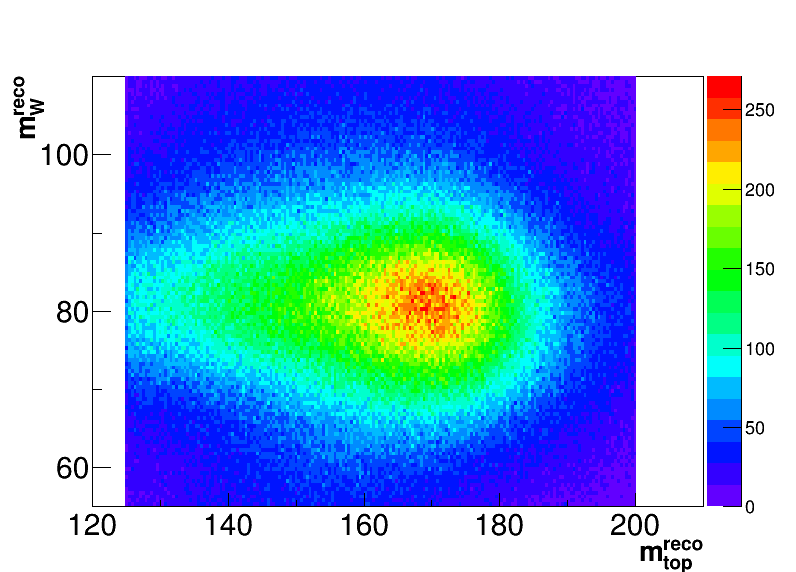
\includegraphics[width=\linewidth]{Pics/PlotCombi/mtopmw.png}
		\caption{Correlation: $m_{top}^{reco}$ and $R_{bq}^{reco}$.} \label{fig:1a}
	\end{subfigure}
	\hspace*{0.1cm}
	\begin{subfigure}{0.4\textwidth}
	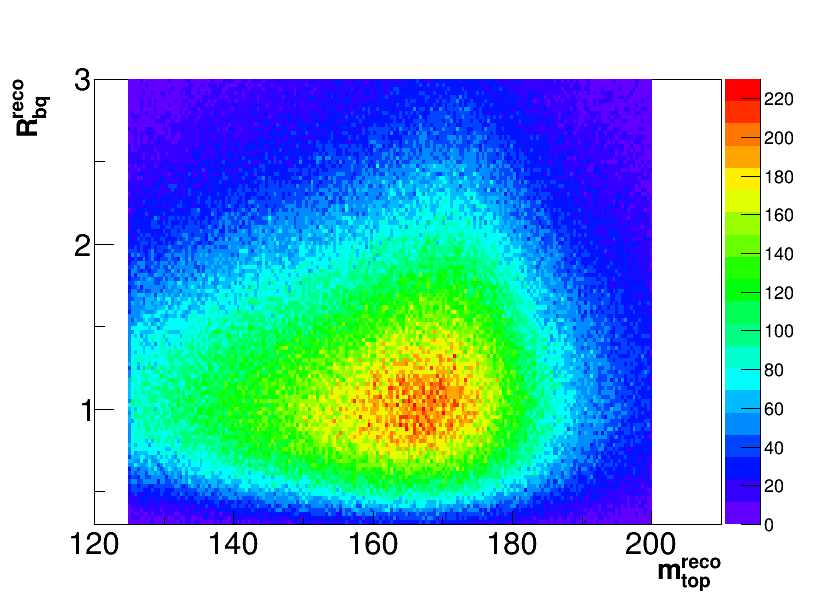
\includegraphics[width=\linewidth]{Pics/PlotCombi/mtopRbq.png}
	\caption{Correlation:  $m_{top}^{reco}$ and $m_{W}^{reco}$.} \label{fig:1b}
	\end{subfigure}

	\begin{subfigure}{0.4\textwidth}
	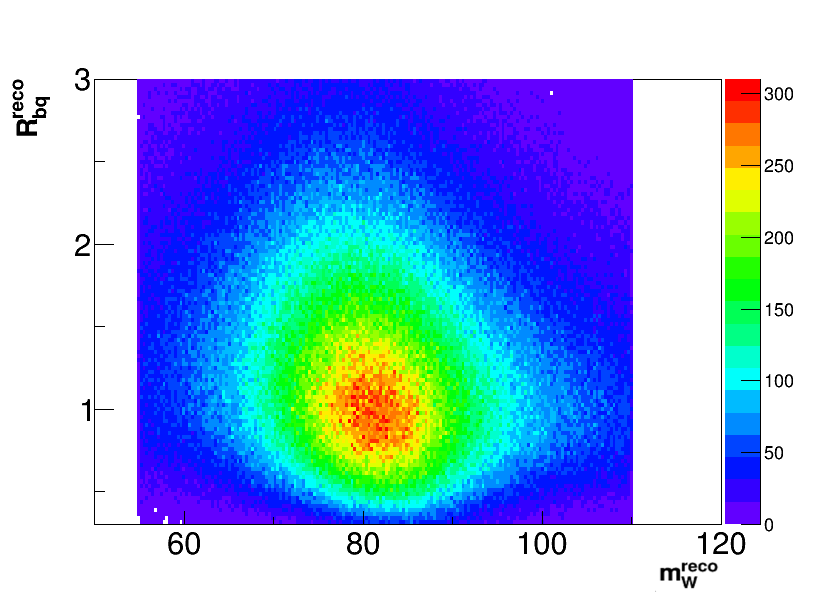
\includegraphics[width=\linewidth]{Pics/PlotCombi/mwRbq2.png}
	\caption{Correlation:  $m_{W}^{reco}$ and $R_{bq}^{reco}$.} \label{fig:1c}
	\end{subfigure}

	\caption{Pair-wise correlation for the observables.}
\end{figure}	


 
 For the determination of the correlation coefficients here,  the entries of the three estimators are plotted against each other  (see~\cref{fig:1a,fig:1b}). $\rho$ is evaluated by counting the entries of this two dimensional plots. As a result one gets the three correlation factors: 
\begin{eqnarray*}
\rho (m_{\text{top}}^{\rm reco} - m_\text{W}^{\rm reco}) = -0.02,\hspace{0.3cm}\rho (m_{\text{top}}^{\rm reco} - R_{\text{bq}}^{\rm reco}) =0.05 \hspace{0.3cm} \text{and} \hspace{0.3cm}
\rho (m_{\text{W}}^{\rm reco} - R_{\text{bq}}^{\rm reco}) = -0.10.\nonumber \\ 
\end{eqnarray*}
Compared to the correlation values which are obtained for the previous measurements, the obtained results are of the same order. Therefore, the here presented correlations are assumed to be  sufficiently small, which allows the application of the factorization theorem. 

 The final likelihood function is:
\begin{eqnarray}
\Likeljets(\mt, \JSF, \bJSF)  &=& 
\prod_{i=1}^{N} P_{\text{top}}(m_{\text{top}}^{\rm reco,i}\,\vert\,\mt, \JSF, \bJSF)\cdot \nonumber \\ &&\quad\quad P_W(m_{\text{W}}^{\rm reco,i}\,\vert\,\JSF)\cdot \nonumber \\ 
 \vspace{0.1cm}
&&\quad\quad P_{R_{\text{bq}}}(R_{\text{bq}}^{\rm reco,i}\,\vert\,\mt,\JSF,\bJSF).
\label{eq:LikeLJ1} 
\end{eqnarray}

The likelihood is a product of probability density functions $P_k$  with $k = $ top, W, R$_{\text{bq}}$, which runs over all $N$ events. The shapes of the three probability densities are obtained from the functional forms of the template parametrization.  $P_{\text{top}}(m_{\text{top}}}^{\rm reco,i}\,\vert\,\mt, \JSF, \bJSF)$ corresponds to the  $m_{\text{top}}^{\rm reco}$ distribution, which is parametrized in $\mt,\JSF $ and $\bJSF$ like $P_{R_{\text{bq}}}(R_{\text{bq}}^{\rm reco,i}\,\vert\,\mt,\JSF,\bJSF)$, the probability density function of $R_{\text{bq}}^{\rm reco}$. 
The probability density function of the $m_{\text{W}}}^{\rm reco}$ distribution  $P_{\text{W}}(m_{\text{W}}}^{\rm reco,i}\,\vert\, \JSF)$ is only parametrized in JSF.  In  this thesis, the probability density functions are representing the signal distributions, without the single top-quark samples. With the minimization of the likelihood, $m_{\text{top}$, JSF and bJSF are determined, which is in the following called three dimensional fit, respectively two and one dimensional fits denote the determination of 
$m_{\text{top}$ and JSF or only of $m_{\text{top}$.


For the previous top-quark mass measurements in the lepton + jets channel, also the background templates are parametrized and taken into account by additional probability functions. In addition to $m_{\text{top}}$, JSF and bJSF,  also the background fraction $f_{bkg}$ is determined with the maximum likelihood fit.  In that case, the corresponding probability density functions take the following form: 

\begin{eqnarray}
	P_{\rm top}(\mtri\,\vert\,\mt, \JSF, \bJSF, \fbkg) &=& 
	(1-\fbkg)\cdot\Ptopsig(\mtri\,\vert\,\mt, \JSF, \bJSF) +
	\nonumber \\&&\quad\quad\,
	\fbkg\cdot\Ptopbkg(\mtri\,\vert\,\JSF, \bJSF)\,\,,
	\nonumber \\
	P_W(m_{\text{W}}^{\rm reco,i}\,\vert\,\JSF, \fbkg) &=& (1-\fbkg)\cdot P_{m_{\text{W}}}^{\text{sig}}(m_{\text{W}}^{\rm reco,i}\,\vert\,\JSF) +
	\nonumber \\
	&& \quad\quad\, \fbkg\cdot P_{\text{W}}^{\text{bkg}}(m_{\text{W}}^{\rm reco,i}\vert\,\JSF)
	\,\,,\nonumber \\
	P_{R_{\text{bq}}}(\rlbri\,\vert\,\mt,JSF,\bJSF, \fbkg)
	&=& (1-\fbkg)\cdot P_{R_{\text{bq}}}^{\text{sig}}(\rlbri \,\vert \mt,\JSF,\bJSF) +
	\nonumber \\
	&& \quad\quad\, \fbkg\cdot P_{R_{\text{bq}}}^{\text{bkg}}(\rlbri\,\vert\,\bJSF).\nonumber \\
		\nonumber \\
\end{eqnarray}




\section{Closure tests}\label{ct}
The Method performance and the consistency of the estimated properties are tested via closure tests. 
Ensembles for each parameter set (m$_{\text{top}}$, JSF, bJSF) are drawn from pseudodata, generated by randomly chosen events from the available Monte Carlo simulation. Each of the generated ensembles corresponds to the integrated luminosity of the data.  
 Bootstrapping~\cite{efron1992bootstrap} is applied to resample the events after their selection. Therefore, one event can appear in several ensembles, which makes it necessary to take care of unwanted correlations among the different ensembles by ensuring that there is enough Monte Carlo statistics or, like for the previous analyses, apply an oversampling correction~\cite{barlow2000application}. 
However, since in this thesis the whole closure test procedure is performed for the first time with the new analyses framework, the oversampling correction is not applied yet.  

With the pseudodata the  unbinned maximum likelihood fit is performed to determine the top-quark mass and the jet energy scale factors. The whole procedure, 
from drawing the pseudoexperiments to the unbinned maximum likelihood fit is performed 250 times. 

For each of the ensembles, $m_{\text{top}}$, JSF and bJSF are obtained and histogrammized. The corresponding expectation values of these distributions are calculated and used to test the linearity of the fit. Therefore, the pseudoexperiments are performed in one, two and three dimensions for the five different input values of $m_{\text{top}}^{\rm in}$, JSF$^{\rm in}$ and bJSF$^{\rm in}$. 
The tests are performed with variing either $m_{\text{top}}$, JSF or bJSF, and keeping the other two fixed to their nominal values. 
For the three-dimensional fit all three variables are varied, in two dimensions, only $m_{\text{top}}^{\rm in}$ and JSF$^{\rm in}$ are considered and in the one dimensional fit only  $m_{\text{top}}^{\rm in}$ is varied. 

  
 Closure tests are performed for each dimension. The difference between the input and the output value of the three variables, i.e.  $m_{\text{top}}^{\rm fit}-m_{\text{top}}^{\rm in}$  (analogous for JSF and bJSF) , are  plotted versus the different input values of $m_{\text{top}}^{\rm in}$, JSF$^{\rm in}$ and bJSF$^{\rm in}$. Moreover,  a linear fit is performed, which takes the statistical uncertainties per parameter into account. The slope of the linear fit is forced to be zero. If the offset of the linear fit is consistent with zero, the result is unbiased.
 
 \begin{figure}[h] % "[t!]" placement specifier just for this example
 	\centering 
 	\begin{subfigure}{0.37\textwidth}
 		\includegraphics[width=\linewidth]{Pics/{Closure_mtop_diff_250PE_1D}.pdf}
 		\label{fig:x1cb}
 	\end{subfigure}	
 	\begin{subfigure}{0.37\textwidth}
 		\includegraphics[width=\linewidth]{Pics/{Closure_mtop_pull_250PE_1D}.pdf}
 		\label{figx:1cb}
 	\end{subfigure}
 	\caption{ 
 		Results of the 1D closure tests. On the right,  $m_{\text{top}}^{\rm fit}$ is plotted vs five different $m_{\text{top}}^{\rm in}$, while  JSF and bJSF are set to 1.00. The results are obtained with 250 pseudoexperiments. In addition, the corresponding pull-widths are shown. The dashed lines represent the ideal value. All error bars correspond to statistical uncertainties. 
 	}\label{closure3}
 \end{figure}
 
 %The consistency of the method is further check by performing cross-checks of the closure tests, i.e. the mass residual is also plotted vs JSF$^{in}$, in the 2D fit and vs bJSF$^{in}$ for the 3D case.\\
 
 
  In addition to the linearity tests, the so-called pull distributions are evaluated by taking also into account the uncertainties of each pseudoexperiment, e.g. $\delta_{m_{\text{top}}^{\rm fit}$. The pull distribution  values for $m_{\text{top}}$ are calculated with:  
 \begin{equation}
 m_{\text{top pull}} = \frac{m_{\text{top}}^{\rm in} - m_{\text{top}}^{\rm fit}}{\delta_{m_{\text{top}}}^{\rm fit}}.
 \end{equation}
 The equation can easily be adapted for the JSF and the bJSF by replacing the corresponding quantities. The pull distribution is evaluated for each variation of the three input variables. If the uncertainties $\delta^{\rm fit}$ are correctly estimated, the width of the pull distributions should be close to unity. Therefore, the  pull-width of each distribution is plotted as a function of the input values ($m_{\text{top}}^{\rm in}$, JSF$^{\rm in}$ and bJSF$^{\rm in}$). A straight line fit provides  the quality of the error estimations. If the uncertainties are underestimated, i.e. the average pull width is too small, the fitted line has a positive offset. Hence, if a negative offset is observed  the  average pull-width is larger than one and  the uncertainties are overestimated.









The results of the one dimensional closure test can be seen, together with the corresponding pull-width plot (right), in~\cref{closure3}. For the linearity test on the left, only $m_{\text{top}}$ is fitted, while both scale factors are set to 1.00.  The result of the linear  fit on the left, demonstrates that the offset is not consistent with zero, but very small. The corresponding pull-width fit, however, shows a noticeable offset from unity towards larger values. Thus, the average pull-width for the different mass points is larger than one and the uncertainties are underestimated.
In~\cref{closure2} the results for the two-dimensional fit are presented. In the top line, the closure tests are displayed for the fit of $m_{\text{top}}$ and JSF. bJSF is kept at 1.00. The second line displays the pull-widths. For the two-dimensional fit, a similar result as in one dimension is obtained. While the linearity tests of $m_{\text{top}}$ and JSF show that the offsets are not consistent with zero, but very small.  The pull-widths show that the uncertainties are underestimated.

\begin{figure} [h]% "[t!]" placement specifier just for this example
	\centering 
	
	\begin{subfigure}{0.35\textwidth}
		\includegraphics[width=\linewidth]{Pics/{Closure_mtop_diff_250PE_2D}.pdf}
		\label{fig:12cb}
	\end{subfigure}	
	\hspace*{0.25cm}
	\begin{subfigure}{0.35\textwidth}
		\includegraphics[width=\linewidth]{Pics/{Closure_jsf_diff_250PE_2D}.pdf}
		\label{fig:21cb}
	\end{subfigure}	
	
	\begin{subfigure}{0.35\textwidth}
		\includegraphics[width=\linewidth]{Pics/{Closure_mtop_pull_250PE_2D}.pdf}
		\label{fig:1cm}
	\end{subfigure}
	\hspace*{0.25cm}
	\begin{subfigure}{0.35\textwidth}
		\includegraphics[width=\linewidth]{Pics/{Closure_jsf_pull_250PE_2D}.pdf}
		\label{fig:1cj}
	\end{subfigure}
	
	
	
	\caption{ 
		The same results as in ~\cref{closure3} are displayed for the two-dimensional fit. The top line shows the closure fits for the top-quark mass and JSF. The bottom line displays the corresponding pull distributions.
	}\label{closure2}
\end{figure}	


 The results of the closure tests and the pull-widths for the three-dimensional fit of $m_{\text{top}}$, JSF and bJSF are presented in~\cref{closure1}. In contrast to the one and two-dimensional closure test, the consistency can not be seen for three dimensions, since the offset in the corresponding plots for $m_{\text{top}}$ and bJSF shows that there is  a bias. Furthermore, the offsets observed for pull-widths show, like for the one and two-dimensional case, that the corresponding uncertainties are underestimated.

   
  The reason for the observed bias in three dimensions might arise due to an insufficient description of the \rm reconstructed distributions by the chosen  parametrization of the templates. In the first runs of the closure test, the linearity tests also failed for the one and two-dimensional fit. This issue could be solved by optimizing the  initial parameters of the simultaneous template parametrization. Therefore, the  further optimization of the simultaneous fit might improve the result of the 3D closure test as well.  In case of the general underestimation of the uncertainties, which is observed for all three dimensions, the corresponding uncertainties have to be studied explicitly. 
  Since only a small offset was observed for the one- and two-dimensional template method, the next analysis step, the evaluation of the systematic uncertainties, takes only the reduced number of dimensions into account.









\begin{landscape}
\begin{figure} % "[t!]" placement specifier just for this example
	\centering 
	\begin{subfigure}{0.37\textwidth}
	\includegraphics[width=\linewidth]{Pics/{Closure_mtop_diff_250PE_3D}.pdf}
 \label{fig:3cm}
	\end{subfigure}
	\hspace*{0.25cm}
	\begin{subfigure}{0.37\textwidth}
	\includegraphics[width=\linewidth]{Pics/{Closure_jsf_diff_250PE_3D}.pdf}
\label{fig:3cj}
	\end{subfigure}
	\hspace*{0.25cm}
	\begin{subfigure}{0.37\textwidth}
	\includegraphics[width=\linewidth]{Pics/{Closure_bjsf_diff_250PE_3D}.pdf}
\label{fig:3cb}
	\end{subfigure}


	\begin{subfigure}{0.37\textwidth}
	\includegraphics[width=\linewidth]{Pics/{Closure_mtop_pull_250PE_3D}.pdf}
\label{fig:3pull1}
	\end{subfigure}
	\hspace*{0.25cm}
	\begin{subfigure}{0.37\textwidth}
	\includegraphics[width=\linewidth]{Pics/{Closure_jsf_pull_250PE_3D}.pdf}
	\label{fig:3pull2}
	\end{subfigure}
	\hspace*{0.25cm}
	\begin{subfigure}{0.37\textwidth}
	\includegraphics[width=\linewidth]{Pics/{Closure_bjsf_pull_250PE_3D}.pdf}
	 \label{fig:3pull3}
	\end{subfigure}
	
	
	

	\caption{
	The same results as in ~\cref{closure3} are displayed for the three dimensional fit. The top line shows the closure fits for the top-quark mass,  JSF and bJSF. The bottom line displays the corresponding pull distributions.
}\label{closure1}
\end{figure}

	
\end{landscape}






